%!TEX program = xelatex
% 完整编译: xelatex -> biber/bibtex -> xelatex -> xelatex
\documentclass[lang=cn,11pt,a4paper]{elegantpaper}

\title{geometry.h文档说明(上)}
\author{Haochen Huang}
\institute{西安交通大学MFM课题组}

\version{1.02test}
\date{\zhtoday}


% 本文档命令
\usepackage{array}

\begin{document}

\maketitle
\tableofcontents

\begin{abstract}
本文为geometry.h的文档说明,该头文件的目的在于为Basilisk提供一些精巧的几何工具,以便为之后的多相流算法(例如VOF算法等)提供工具支持。由于本文件工具种类繁多,现暂分上下两部,上部中为常用,最值得注意的相关函数。下部则是部分辅助输出函数。\par
2.02版本更新,解决内部排版问题,增改部分注释
\end{abstract}

\section{文件中主要函数及其目的}
\subsection{文件目的}
以一个被两相边界分割的2D单元为例:\par
\begin{figure}[H]
\begin{center}
    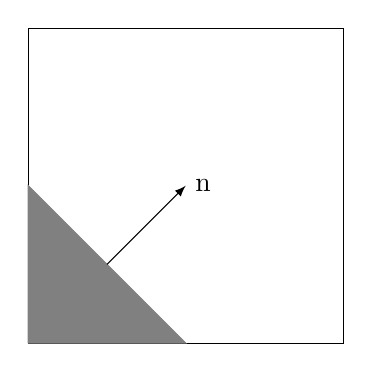
\begin{tikzpicture}[scale=1]
    \draw (-2,0)--(2,0)--(2,4)--(-2,4)--(-2,0);
    \filldraw[gray] (-2,0)--(-2,2)--(0,0)--(-2,0);
    \draw[-latex](-1,1)--(0,2) node[anchor=west]{n};
    \end{tikzpicture}
\end{center}
\caption{2D示例单元}
\end{figure}
其中灰色部分代表边界内,白色部分代表边界外,边界的法向量统一指向外侧。假设两相边界的方程为
\begin{equation}
    n_xx+n_yy=\alpha
\end{equation}
其中$n_x,n_y$为单位化后法向量的两个分量,我们由此引入描述边界的三个参数:
\begin{itemize}
    \item 表示边界内所占该单元体积面积的体积分数c
    \item 边界的法向量$(n_x,n_y)$(三维则为$(n_x,n_y,n_z)$)
    \item 以及边界函数表达中的参数$\alpha$
\end{itemize}
此三者并非相互独立,在已知边界法向量以及剩下两者中的一者后,可以轻易的推导出余下一个参数,而本头文件中的工具就是针对该问题进行一系列的求解。\par
\subsection{主要函数}
\begin{itemize}
    \item line alpha/plane alpha:用于求解2维/3维情况下已知体积占比$c$以及边界法向量$n$时,该边界在本单元中的参数$\alpha$
    \item line area/plane area:用于求解2维/3维情况下已知界面参数$\alpha$以及边界法向量$n$时,该边界在本单元中的面积/体积分数$c$
    \item rectangle fraction:用于求解网格内方形部分的边界内体积/面积分数$c$
    \item facets:用于输出界面端点坐标,在后处理中可以将端点坐标用直线连接
    \item line length center/plane area center:用于存储2维/3维中边界中心,同时输出边界内部在单元中的面积/体积
    \item line center/plane center:用于输出边界内面积体积重心坐标
\end{itemize}
\section{line alpha/plane alpha函数}
\subsection{函数目的及原理}
该函数目的是在给定界面法向量$(n_x,n_y)$以及界面内体积占比$c$后计算界面参数$\alpha$。\par
算法重点在于坐标转换以及临界面积推导;其中坐标转换会在下一节详细阐述,本节主要讲解面积推导。\par
我们首先将原本的坐标及图形经历坐标变换全部变为零点在左下角,法向量分量均大于零的状态,见\ref{fig:pianyi},具体推到公式及返回见下一节。\par
当$c\in (0,1)$,且$n_x,n_y$均不等于0时,为了方便区分,算法将分量中较大的一个定义为$n_2$,较小的一个定义为$n_1$,我们以$n_y$为较大数为例,有:\par
\begin{figure}[htbp]
    \centering
    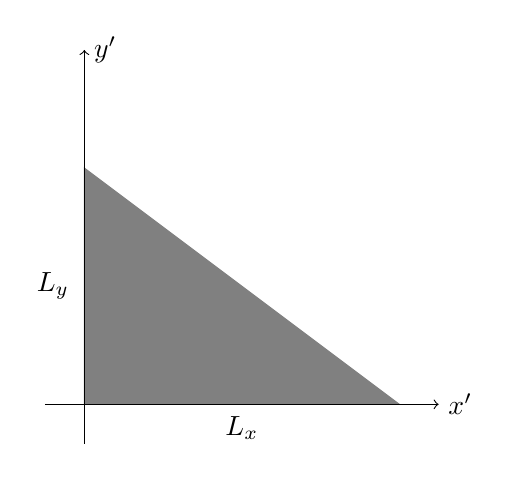
\begin{tikzpicture}[scale=1]
    \filldraw[gray] (-2,0)--(-2,3)--(2,0)--(-2,0);
    \node[left=2pt](a) at (-2,1.5) {$L_y$};
    \node[below=1pt](b) at (0,0) {$L_x$};
    \draw[->] (-2.5,0)--(2.5,0) node[anchor=west]{$x'$};
    \draw[->] (-2.0,-0.5)--(-2.0,4.5) node[anchor=west]{$y'$};
    \end{tikzpicture}
    \caption{界面与两坐标轴的交点}
    \label{fig:jiaodian}
\end{figure}
令落在$x'$轴上的长度为$L_x$,令落在$y'$轴上的长度为$L_y$,则$\frac{L_y}{L_x}=\frac{n_x}{n_y}$,且$L_y\leq L_x$。面积共有三种情况图形一共有三种形态,分别是三角形,梯形,以及五边形,详见\ref{fig:mianjiqingkuang},当前目标是:使用已知的$c$与$(n_x',n_y')$对其进行判定,首先为三角形临界情况:\par
\begin{figure}[htbp]
    \centering
    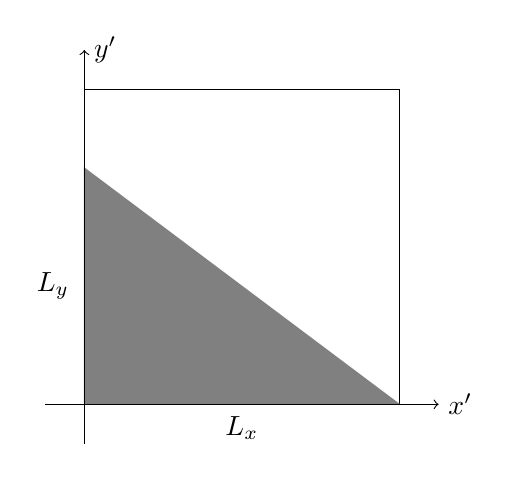
\begin{tikzpicture}[scale=1]
    \draw (-2,0)--(2,0)--(2,4)--(-2,4)--(-2,0);
    \filldraw[gray] (-2,0)--(-2,3)--(2,0)--(-2,0);
    \node[left=2pt](a) at (-2,1.5) {$L_y$};
    \node[below=1pt](b) at (0,0) {$L_x$};
    \draw[->] (-2.5,0)--(2.5,0) node[anchor=west]{$x'$};
    \draw[->] (-2.0,-0.5)--(-2.0,4.5) node[anchor=west]{$y'$};
    \end{tikzpicture}
    \caption{三角形面积临界情况}
    \label{fig:sanjiaomingjilinjie}
\end{figure}
即$L_x=1$此时其面积为:
\begin{equation}
    c = \frac{n_1}{2n_2}
\end{equation}
是故当$c\leq \frac{n_1}{2n_2}$时,图形为三角形,即可以求出$\alpha$,具体公式详见下节。\par
而梯形的临界状态则为:\par
\begin{figure}[htbp]
    \centering
    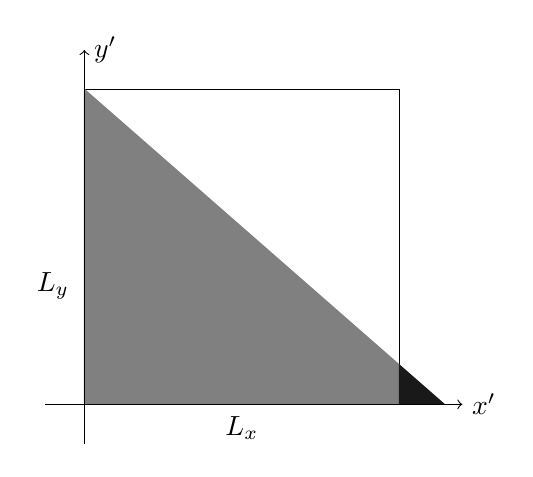
\begin{tikzpicture}[scale=1]
    \draw (-2,0)--(2,0)--(2,4)--(-2,4)--(-2,0);
    \filldraw[gray] (-2,0)--(-2,4)--(2,0.5)--(2,0)--(-2,0);
    \filldraw[gray!20!black] (2,0)--(2,0.5)--(2.5714,0)--(2,0);
    \node[left=2pt](a) at (-2,1.5) {$L_y$};
    \node[below=1pt](b) at (0,0) {$L_x$};
    \draw[->] (-2.5,0)--(2.8,0) node[anchor=west]{$x'$};
    \draw[->] (-2.0,-0.5)--(-2.0,4.5) node[anchor=west]{$y'$};
    \end{tikzpicture}
    \caption{梯形面积临界情况}
    \label{fig:tixingmingjilinjie}
\end{figure}
此时单元内右上角空白三角形的面积为:
\begin{equation}
    S_{blank} = \frac{n_1}{2n_2}
\end{equation}
则当$c\leq 1-\frac{n_1}{2n_2}$时,计算为梯形,则其余均为五边形。相关计算公式同见下节。
\subsection{具体实现代码}
\begin{minted}[mathescape=true,breaklines]{lexer.py:DiffLexer -x}
#if dimension >= 2
double line_alpha (double c, coord n)
{
  double alpha, n1, n2;
  
  n1 = fabs (n.x); n2 = fabs (n.y);
  if (n1 > n2)//判断法向分量中的较大值,并将其赋于$n_2$
    swap (double, n1, n2);

  c = clamp (c, 0., 1.);
  double v1 = n1/2.;
  if (c <= v1/n2)//面积为三角形的判断
    alpha = sqrt (2.*c*n1*n2);//相关$\alpha$计算
  else if (c <= 1. - v1/n2)//梯形判断
    alpha = c*n2 + v1;
  else//五边形判断
    alpha = n1 + n2 - sqrt (2.*n1*n2*(1. - c));
  //坐标反变换
  if (n.x < 0.)
    alpha += n.x;
  if (n.y < 0.)
    alpha += n.y;

  return alpha - (n.x + n.y)/2.;
}
#endif // dimension >= 2

#if dimension >= 3
double plane_alpha (double c, coord n)
{
  double alpha;
  coord n1;
  
  n1.x = fabs (n.x); n1.y = fabs (n.y); n1.z = fabs (n.z);

  double m1, m2, m3;
  m1 = min(n1.x, n1.y);
  m3 = max(n1.x, n1.y);
  m2 = n1.z;
  if (m2 < m1) {
    double tmp = m1;
    m1 = m2;
    m2 = tmp;
  }
  else if (m2 > m3) {
    double tmp = m3;
    m3 = m2;
    m2 = tmp;
  }
  double m12 = m1 + m2;
  double pr = max(6.*m1*m2*m3, 1e-50);
  double V1 = m1*m1*m1/pr;
  double V2 = V1 + (m2 - m1)/(2.*m3), V3;
  double mm;
  if (m3 < m12) {
    mm = m3;
    V3 = (m3*m3*(3.*m12 - m3) + m1*m1*(m1 - 3.*m3) + m2*m2*(m2 - 3.*m3))/pr;
  }
  else {
    mm = m12;
    V3 = mm/(2.*m3);
  }

  c = clamp (c, 0., 1.);
  double ch = min(c, 1. - c);
  if (ch < V1)
    alpha = pow (pr*ch, 1./3.);
  else if (ch < V2)
    alpha = (m1 + sqrt(m1*m1 + 8.*m2*m3*(ch - V1)))/2.;
  else if (ch < V3) {
    double p12 = sqrt (2.*m1*m2);
    double q = 3.*(m12 - 2.*m3*ch)/(4.*p12);
    double teta = acos(clamp(q,-1.,1.))/3.;
    double cs = cos(teta);
    alpha = p12*(sqrt(3.*(1. - cs*cs)) - cs) + m12;
  }
  else if (m12 <= m3)
    alpha = m3*ch + mm/2.;
  else {
    double p = m1*(m2 + m3) + m2*m3 - 1./4., p12 = sqrt(p);
    double q = 3.*m1*m2*m3*(1./2. - ch)/(2.*p*p12);
    double teta = acos(clamp(q,-1.,1.))/3.;
    double cs = cos(teta);
    alpha = p12*(sqrt(3.*(1. - cs*cs)) - cs) + 1./2.;
  }
  if (c > 1./2.) alpha = 1. - alpha;

  if (n.x < 0.)
    alpha += n.x;
  if (n.y < 0.)
    alpha += n.y;
  if (n.z < 0.)
    alpha += n.z;

  return alpha - (n.x + n.y + n.z)/2.;;
}
#else // dimension < 3
# define plane_alpha line_alpha
#endif
\end{minted}
\section{line area/plane area函数}
\subsection{函数目的及原理}
该函数目的是在给定界面的法向量$n_x,n_y$以及界面参数$\alpha$后,求解界面内在单元中的占比。\par
本算法的精髓在于\textbf{坐标变换};依旧以2维为例,法向量的组合共有四种即:$(n_x>0,n_y>0),(n_x>0,n_y<0),(n_x<0,n_y>0),(n_x<0,n_y<0)$,为了简便计算,我们应该在保证图形不发生改变的情况下使用坐标变换,将坐标中心移至左下角,并将法向量变为$(n_x'>0,n_y'>0)$,如下图:\par
\begin{figure}[htbp]
    \centering
    \begin{center}
    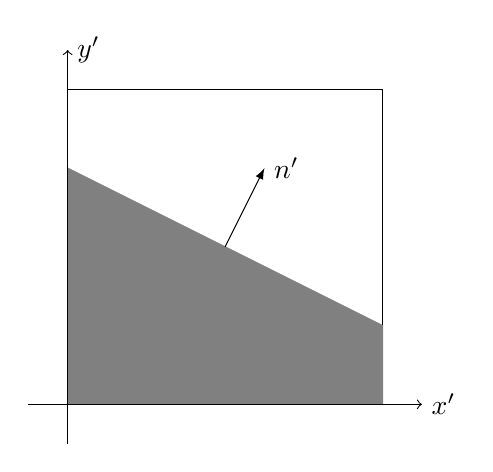
\begin{tikzpicture}[scale=1]
    \draw (-2,0)--(2,0)--(2,4)--(-2,4)--(-2,0);
    \filldraw[gray] (-2,0)--(-2,3)--(2,1)--(2,0)--(-2,0);
    \draw[->] (-2.5,0)--(2.5,0) node[anchor=west]{$x'$};
    \draw[->] (-2.0,-0.5)--(-2.0,4.5) node[anchor=west]{$y'$};
    \draw[-latex](0,2)--(0.5,3) node[anchor=west]{$n'$};
    \end{tikzpicture}
    \end{center}
    \caption{坐标变换示例}
    \label{fig:pianyi1}
\end{figure}
其中$'$表示坐标变换。根本原理如下:\par
有原方程式:
\begin{equation}
    n_xx+n_yy=\alpha
\end{equation}
现将坐标平移至左下,即:
\begin{equation}
    \left\{ 
    \begin{array}{cc}
    x'=&x+\frac{1}{2}\\
    y'=&y+\frac{1}{2}
    \end{array}
    \right.
\end{equation}
则原式变为:
\begin{equation}
    n_xx'+n_yy'=\alpha+\frac{1}{2}(n_x+n_y)
\end{equation}
接下来对法向量进行变换,当法向量两分量均大于零时可以跳过此步,当两分量中有一个小于零时,可以通过使直线关于$x=\frac{1}{2}$或$y=\frac{1}{2}$进行对称,该步骤具有叠加性,现取$n_x<0$为例:\par
\begin{align}
    \frac{1}{2}-x''=&x'-\frac{1}{2}\\
    (1-x'')=&x'
\end{align}
有:\par
\begin{equation}
    -n_xx''+n_yy'=\alpha\frac{n_y-n_x}{2}
\end{equation}
面积计算时,算法将情况同样分为了四种,如下图
\begin{figure}[htbp]
    \centering
    \subfigure[情况1]{
    \begin{minipage}[t]{0.25\linewidth}
    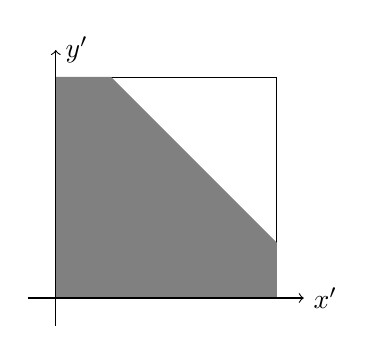
\begin{tikzpicture}[scale=0.7]
    \draw (-2,0)--(2,0)--(2,4)--(-2,4)--(-2,0);
    \filldraw[gray] (-2,0)--(-2,4)--(-1,4)--(2,1)--(2,0)--(-2,0);
    \draw[->] (-2.5,0)--(2.5,0) node[anchor=west]{$x'$};
    \draw[->] (-2.0,-0.5)--(-2.0,4.5) node[anchor=west]{$y'$};
    \end{tikzpicture}
    \end{minipage}
    }
    \subfigure[情况2]{
    \begin{minipage}[t]{0.25\linewidth}
    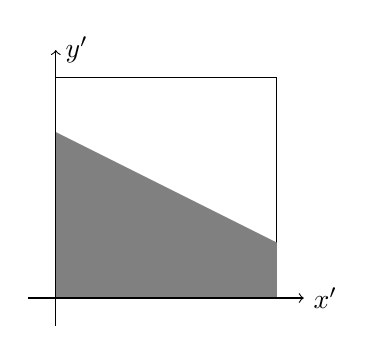
\begin{tikzpicture}[scale=0.7]
    \draw (-2,0)--(2,0)--(2,4)--(-2,4)--(-2,0);
    \filldraw[gray] (-2,0)--(-2,3)--(2,1)--(2,0)--(-2,0);
    \draw[->] (-2.5,0)--(2.5,0) node[anchor=west]{$x'$};
    \draw[->] (-2.0,-0.5)--(-2.0,4.5) node[anchor=west]{$y'$};
    \end{tikzpicture}
    \end{minipage}
    }
    \subfigure[情况3]{
    \begin{minipage}[t]{0.25\linewidth}
    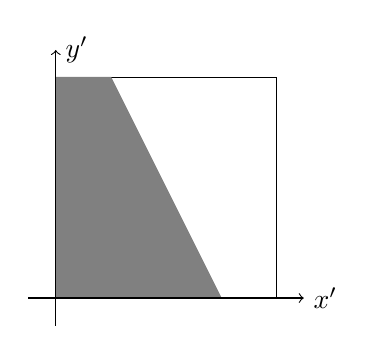
\begin{tikzpicture}[scale=0.7]
    \draw (-2,0)--(2,0)--(2,4)--(-2,4)--(-2,0);
    \filldraw[gray] (-2,0)--(-2,4)--(-1,4)--(1,0)--(-2,0);
    \draw[->] (-2.5,0)--(2.5,0) node[anchor=west]{$x'$};
    \draw[->] (-2.0,-0.5)--(-2.0,4.5) node[anchor=west]{$y'$};
    \end{tikzpicture}
    \end{minipage}
    }
    \subfigure[情况4]{
    \begin{minipage}[t]{0.25\linewidth}
    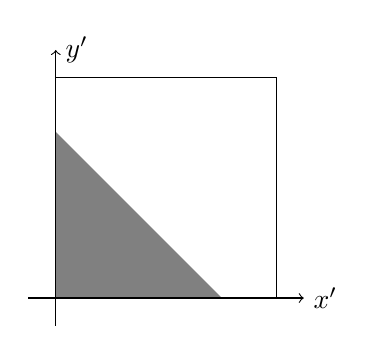
\begin{tikzpicture}[scale=0.7]
    \draw (-2,0)--(2,0)--(2,4)--(-2,4)--(-2,0);
    \filldraw[gray] (-2,0)--(-2,3)--(1,0)--(-2,0);
    \draw[->] (-2.5,0)--(2.5,0) node[anchor=west]{$x'$};
    \draw[->] (-2.0,-0.5)--(-2.0,4.5) node[anchor=west]{$y'$};
    \end{tikzpicture}
    \end{minipage}
    }
    \caption{面积计算中出现的四种情况}
    \label{fig:mianjiqingkuang}
\end{figure}
我们将边界延长至与两对称轴相交,形成三角形,再用三角形减去多余部分即是体积占比,如下图:\par
\begin{figure}[htbp]
    \centering
    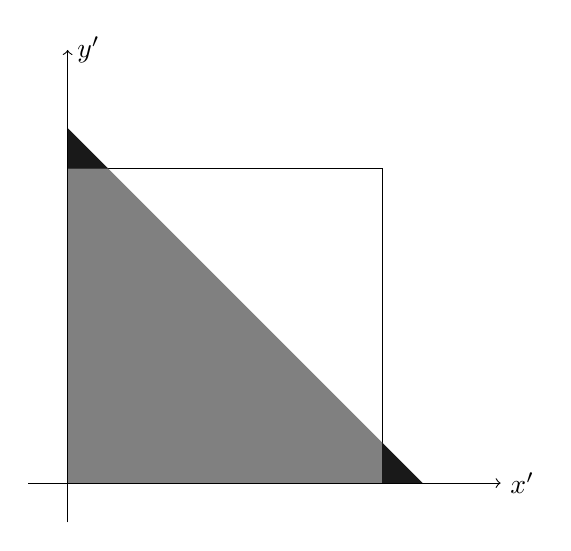
\begin{tikzpicture}[scale=1]
    \draw (-2,0)--(2,0)--(2,4)--(-2,4)--(-2,0);
    \filldraw[gray] (-2,0)--(-2,4)--(-1.5,4)--(2,0.5)--(2,0)--(-2,0);
    \filldraw[gray!20!black] (-2,4)--(-1.5,4)--(-2,4.5)--(-2,4);
    \filldraw[gray!20!black] (2,0)--(2,0.5)--(2.5,0)--(2,0);
    \draw[->] (-2.5,0)--(3.5,0) node[anchor=west]{$x'$};
    \draw[->] (-2.0,-0.5)--(-2.0,5.5) node[anchor=west]{$y'$};
    \end{tikzpicture}
    \caption{面积计算示意}
    \label{fig:mianjijisuan}
\end{figure}
我们可以轻松计算得,大三角形的面积永远为:
\begin{equation}
    S = \frac{\alpha^2}{2n_x'n_y'}
\end{equation}
是故我们只需要判断,图形是否与$x',y'$轴的交点大于1,并减去相应的面积即可,我们依旧以$x'$方向为例:\par
首先判断是否有多余面积,即若:
\begin{equation}
    n_x'(x'-1)+n_y'y'=\alpha - n_x'>0
\end{equation}
则表明其有多余的面积部分,多余面积部分的面积为:
\begin{equation}
    S_r = \frac{(\alpha-n_x')^2}{2n_x'n_y'}
\end{equation}
其余方向同理,减去即可。\par
需要注意的是,形状还有可能是标准的长方形,此时只需要判断斜率,并做简单计算即可。三维与二维的算法原理同理,在此不多做赘述。
\subsection{具体实现代码}
\begin{minted}[mathescape=true,breaklines]{lexer.py:DiffLexer -x}
#if dimension >= 2
double line_area (double nx, double ny, double alpha)
{
  double a, v, area;

  alpha += (nx + ny)/2.;//坐标偏移至左下角
  if (nx < 0.) {//判断法向量分量正负,通过坐标变换全部变为正值
    alpha -= nx;
    nx = - nx;
  }
  if (ny < 0.) {
    alpha -= ny;
    ny = - ny;
  }

  if (alpha <= 0.)//判断单元内是否有界面内部分
    return 0.;

  if (alpha >= nx + ny)//界面过点$(1,1)$为临界状态,代表整个单元均在界面内
    return 1.;

  if (nx < 1e-10)//判断是否为长方形
    area = alpha/ny;
  else if (ny < 1e-10)
    area = alpha/nx;
  else {
    v = sq(alpha);

    a = alpha - nx;//图形是否有多余的三角形面积
    if (a > 0.)
      v -= a*a;
    
    a = alpha - ny;
    if (a > 0.)
      v -= a*a;

    area = v/(2.*nx*ny);
  }

  return clamp (area, 0., 1.);
}
#endif // dimension >= 2

#if dimension >= 3
double plane_volume (coord n, double alpha)
{
  double al = alpha + (n.x + n.y + n.z)/2. +
    max(0., -n.x) + max(0., -n.y) + max(0., -n.z);
  if (al <= 0.)
    return 0.;
  double tmp = fabs(n.x) + fabs(n.y) + fabs(n.z);
  if (al >= tmp)
    return 1.;
  if (tmp < 1e-10)
    return 0.;
  double n1 = fabs(n.x)/tmp;
  double n2 = fabs(n.y)/tmp;
  double n3 = fabs(n.z)/tmp;
  al = max(0., min(1., al/tmp));
  double al0 = min(al, 1. - al);
  double b1 = min(n1, n2);
  double b3 = max(n1, n2);
  double b2 = n3;
  if (b2 < b1) {
    tmp = b1;
    b1 = b2;
    b2 = tmp;
  }
  else if (b2 > b3) {
    tmp = b3;
    b3 = b2;
    b2 = tmp;
  }
  double b12 = b1 + b2;
  double bm = min(b12, b3);
  double pr = max(6.*b1*b2*b3, 1e-50);
  if (al0 < b1)
    tmp = al0*al0*al0/pr;
  else if (al0 < b2)
    tmp = 0.5*al0*(al0 - b1)/(b2*b3) +  b1*b1*b1/pr;
  else if (al0 < bm)
    tmp = (al0*al0*(3.*b12 - al0) + b1*b1*(b1 - 3.*al0) +
	   b2*b2*(b2 - 3.*al0))/pr;
  else if (b12 < b3)
    tmp = (al0 - 0.5*bm)/b3;
  else
    tmp = (al0*al0*(3. - 2.*al0) + b1*b1*(b1 - 3.*al0) + 
	   b2*b2*(b2 - 3.*al0) + b3*b3*(b3 - 3.*al0))/pr;

  double volume = al <= 0.5 ? tmp : 1. - tmp;
  return clamp (volume, 0., 1.);
}
#else // dimension < 3
# define plane_volume(n, alpha) line_area(n.x, n.y, alpha)
#endif
\end{minted}
\section{rectangle fraction函数}
\subsection{函数目的及原理}
如下图:\par
\begin{figure}[htbp]
    \centering
    \begin{center}
    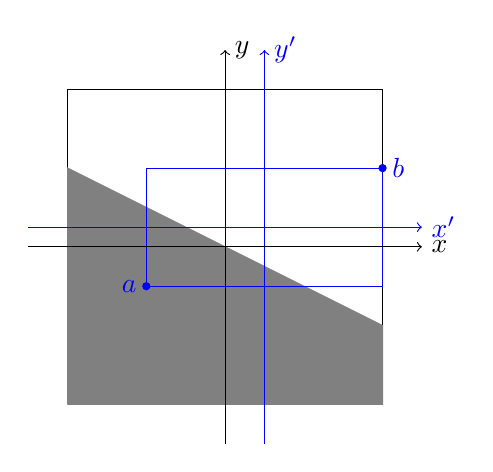
\begin{tikzpicture}[scale=1]
    \draw (-2,0)--(2,0)--(2,4)--(-2,4)--(-2,0);
    \filldraw[gray] (-2,0)--(-2,3)--(2,1)--(2,0)--(-2,0);
    \draw[blue] (-1,1.5)--(-1,3)--(2,3)--(2,1.5)--(-1,1.5);
    \fill[blue] (2,3) circle (1.5pt) node[anchor=west]{$b$};
    \fill[blue] (-1,1.5) circle (1.5pt) node[anchor=east]{$a$};
    \draw[blue,->] (-2.5,2.25)--(2.5,2.25) node[anchor=west]{$x'$};
    \draw[blue,->] (0.5,-0.5)--(0.5,4.5) node[anchor=west]{$y'$};
    \draw[->] (-2.5,2)--(2.5,2) node[anchor=west]{$x$};
    \draw[->] (0,-0.5)--(0,4.5) node[anchor=west]{$y$};
    \end{tikzpicture}
    \end{center}
    \caption{偏移坐标变换示例}
    \label{fig:pianyi}
\end{figure}

该函数的目的在于在原本单元中给定两点$a,b$构成一个新的直角单元网格,通过在原单元中的边界法向量$n$,以及边界参数$\alpha$计算在变形单元中的面积/体积占比。\par
对原坐标进行坐标变换有
\begin{equation}
    \left\{
    \begin{array}{cc}
    x'=&(x_b-x_a)x-\frac{x_b+x_a}{2}\\
    y'=&(y_b-y_a)y-\frac{y_b+y_a}{2} 
    \end{array}
    \right.
\end{equation}
即可得到在该坐标中:
\begin{align}
\alpha ' =& \alpha - n_x\cdot (x_b+x_a)/2 - n_y\cdot (y_b+y_a)/2\\
n'=& (n_x\cdot (x_b-x_a),n_y\cdot (y_b-y_a))
\end{align}
值得注意的是,改代码将直角单元长宽缩放转化为了正方形单元,我们再使用函数plane volume进行面积占比计算,这一操作并不会影响结果。
\subsection{具体实现代码}
\begin{minted}[mathescape=true,breaklines]{lexer.py:DiffLexer -x}
double rectangle_fraction (coord n, double alpha, coord a, coord b)
{
  coord n1;
  foreach_dimension() {
    alpha -= n.x*(b.x + a.x)/2.;
    n1.x = n.x*(b.x - a.x);
  }
  return plane_volume (n1, alpha);
}
\end{minted}
1111


单行代码展示\mintinline{lexer.py:DiffLexer -x}{double un = dt*uf.x[]/(fm.x[]*Delta + SEPS), s = sign(un);} 
\end{document}